%%This is a very basic article template.
%%There is just one section and two subsections.
\documentclass[times,10pt,twocolumn,letterpaper]{article}
\usepackage{color}
\usepackage{ncvpripg}
\usepackage{times}
\usepackage[pdftex]{graphicx}	
\usepackage[cmex10]{amsmath}
\usepackage{url} 

\title{Stagnant Water Detection Using quadcopter}
\author{}
\def\iccvPaperID{238}
\begin{document}
\maketitle

\begin{abstract}
Recently, in urban areas there has been a sharp increase in dengue and malaria.
One of the major reason for this is suspected to be the amount of stagnant
water around residencies. There are many areas around urban residential places
such as terraces of high rise buildings, and shades above windows
(popularly known as `chhajja') that are hard to reach and hence to inspect. We
used quadcopter to inspect such areas and detect whether there is stagnant
water.

\end{abstract}

\section{Introduction}
{\color{red} [MGP] Need to cut short the introduction}

Dengue~\cite{WHO15Dengue} and Malaria~\cite{WHO15Malaria} are among the deadly
diseases common in at least 100 countries in Asia, the Pacific, the Americas,
Africa, and the Caribbean. In India itself there are around one million Malaria
cases ~\cite{NVBDP_Malaria} and fourty thousand cases of dengue
~\cite{NVBDP_Dengue} in year 2014. The disease is transmitted by the biting of
mosquitoes and if not appropriately treated, people may have recurrences of the
disease months later \cite{Cecilia14}. These mosquitoes flourish during rainy seasons but can breed
in water-filled flower pots, plastic bags, and cans year-round. Stagnant water
is major site for breeding of these mosquitoes.

The risk of disease can be reduced by preventing mosquito bites by using
mosquito nets and insect repellents, or with mosquito-control measures such as
spraying insecticides and draining standing water.  Even though major measures
are in exercise since 90’s till now, we have not succeeded in eradicating these
diseases. One of the major reasons behind this is existence of water-puddles
around urban residential places.

Some areas such as high rise buildings' terraces, construction sites, area
near water storage (having possible leakages/overflows) etc. does not attract
attention easily. So, we need an effective mechanism to keep an ``eye'' on such
areas to detect presence of stagnant water. 

Microsoft \cite{Microsoft15} have started ``Project Premonition'' which aims to
use drones to catch mosquitoes for detection of pathogens in them before these
pathogens make people sick. But for sending drones to catch mosquitoes we first
need to find out possible mosquito breeding areas such as water puddles. We
propose a method in which we manuevere a quadcopter to record video of the
whole place, and later process that video to identify the frames which contain
water puddle, which will in turn aid in the process of identifying particular
areas for further action.

\begin{figure}[h!]
\centering
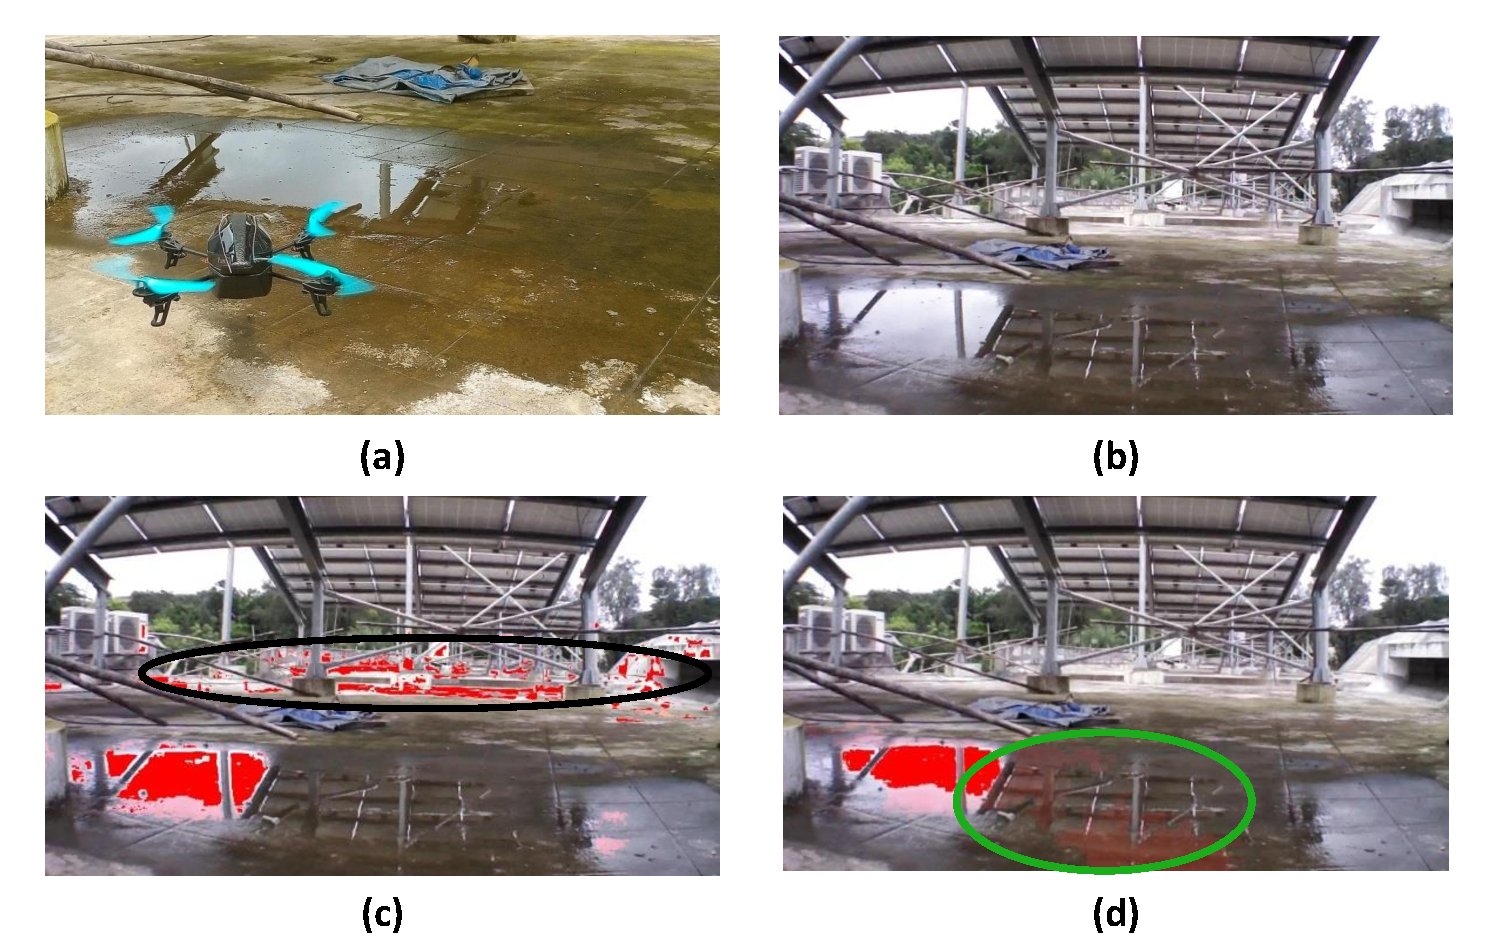
\includegraphics[width=\linewidth]{images/teaser.pdf}
\caption{(a) Quadcopter hovering over stagnant water amassed at building
backyard. (b) Scene captured by quadcopter (c) Our algorithm is able to detect
puddle region in the scene (shown in red).}
\end{figure}

\section{Related Work}

Rankin et al.~\cite{rankin04} have detected the presence of water from color,
texture, and the detection of reflections in stereo range data. They have used a
rule base for fusing water cues which was developed by evaluating detection
results from an extensive archive of data collection imagery containing water.
In another work, Rankin et al.~\cite{rankin11} have implemented a water detector
based on sky reflections that geometrically locates the pixel in the sky that
is reflecting on a candidate water pixel on the ground and predicts if the
ground pixel is water based on color similarity and local terrain features. 

Santana et al.~\cite{santana12}'s method for detection of water relies on the
chaotic nature of water’s dynamic texture to exploit a measure of entropy over the
trajectories obtained from optical flow trackers over several frames.

Zhang et al.~\cite{zhang10} have introduced a descriptor which is tolerant
to the flip transformation and even non-rigid distortions, such as ripple
effects (in additon to invariant to scales, rotations and affine
transformations) to detect water reflections.

\section{Methodology}
In this section we will see the three approaches; SVM classifier with HSV
histogram based feature, Optical flow based technique, and finally combination
of these two approaches to detect stagnant water robustly.

\subsection{SVM classifier}

\begin{figure}[h!]
\centering
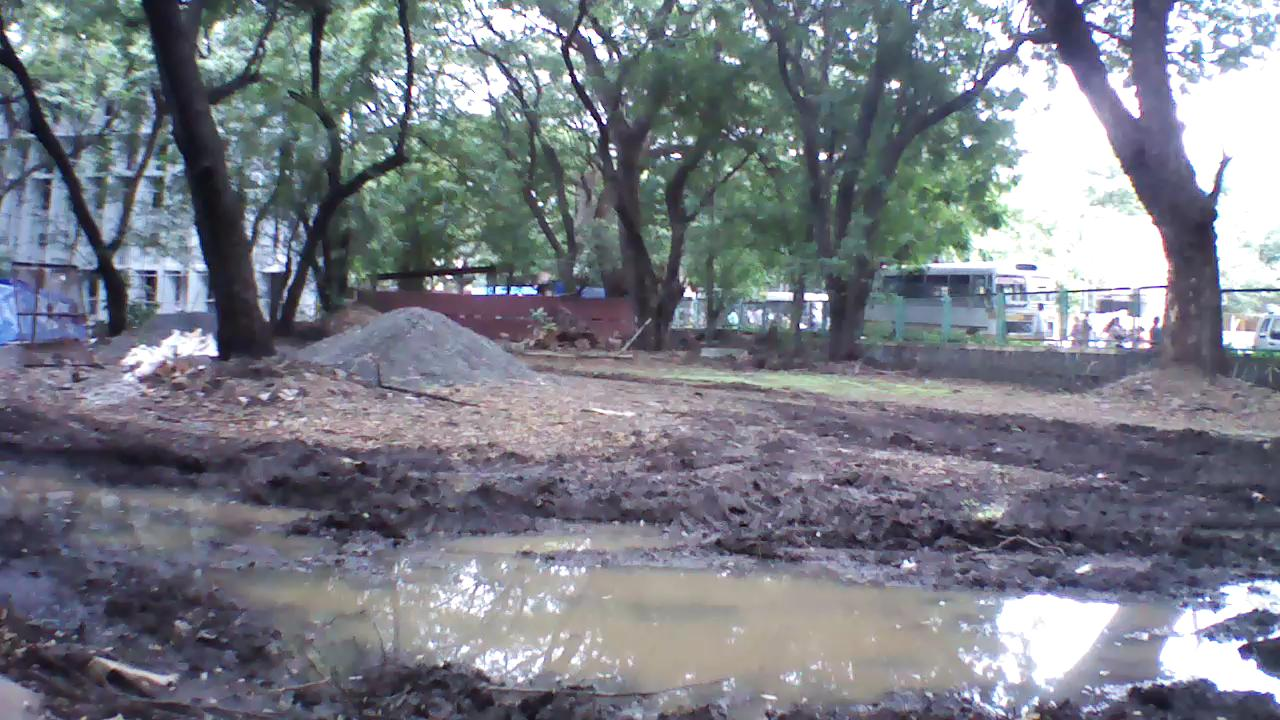
\includegraphics[width=0.22\linewidth]{images/IMG_PAIR_1_1.jpg}
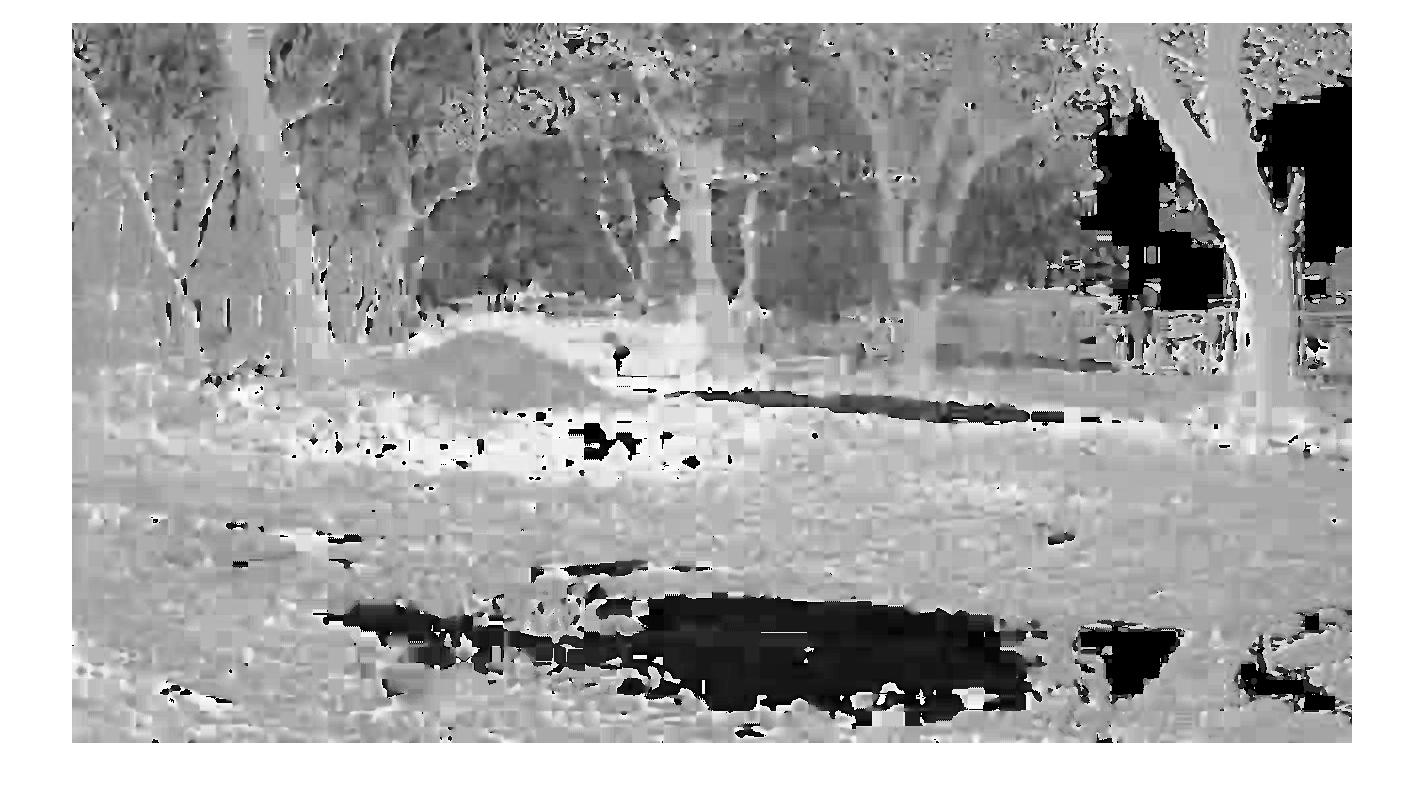
\includegraphics[width=0.22\linewidth]{images/IMG_PAIR_1_1_H.jpg}
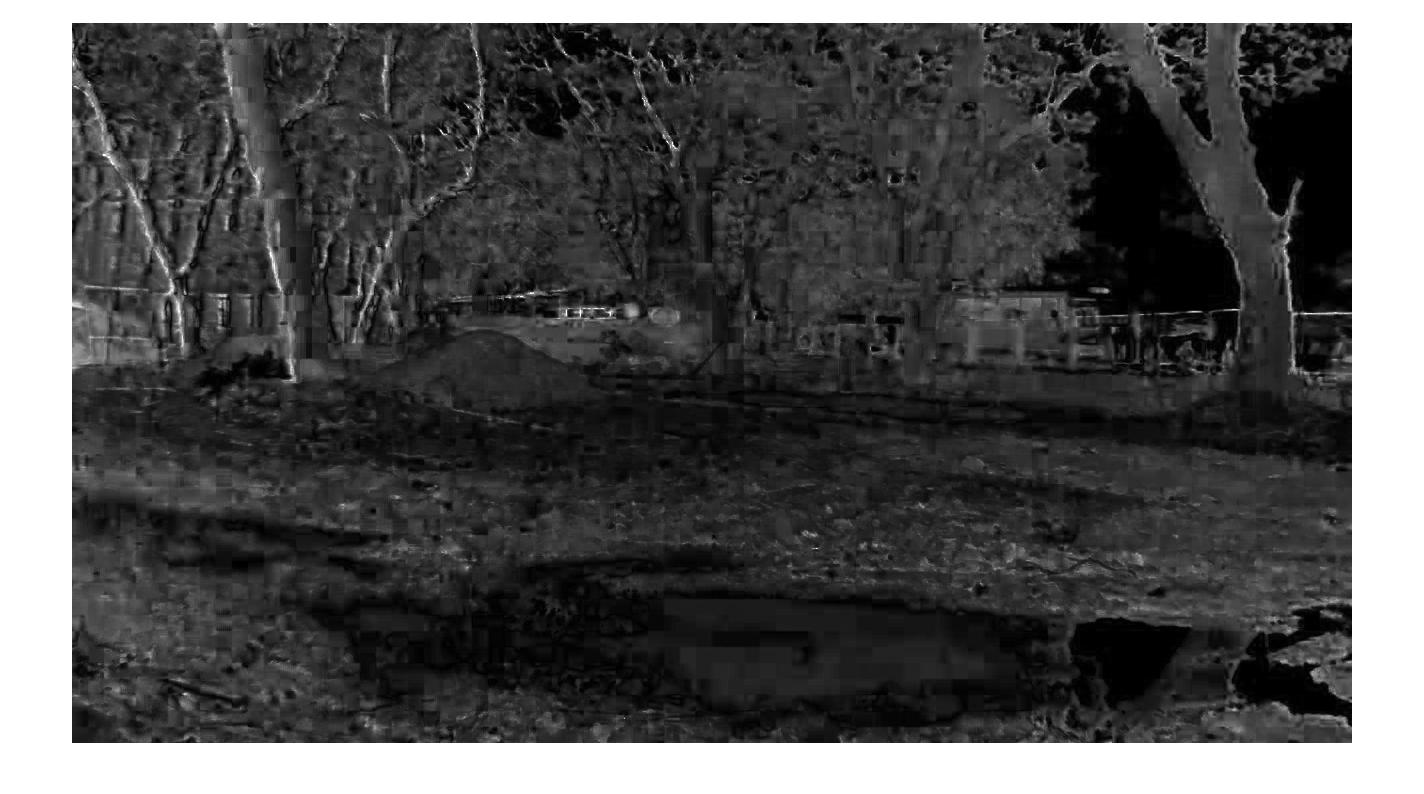
\includegraphics[width=0.22\linewidth]{images/IMG_PAIR_1_1_S.jpg}
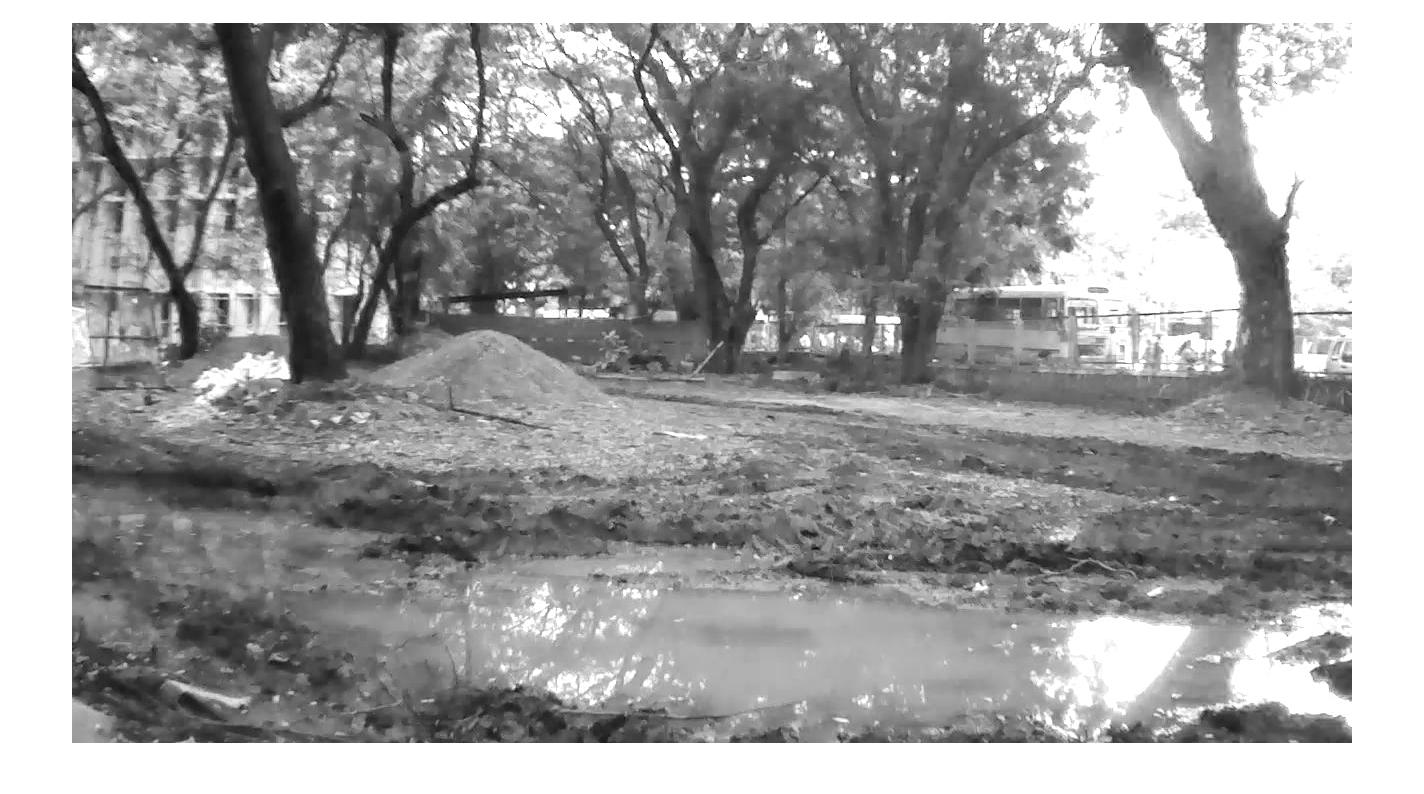
\includegraphics[width=0.22\linewidth]{images/IMG_PAIR_1_1_V.jpg}
\caption{Sample image and their Hue (H), Saturation (S) and Value (V) components
respectively. It can be seen that puddle area has very less Hue as well
as Saturation. Also, reflective parts of puddle has high intensity.}
\label{fig:HSV}
\end{figure}

Under ambient lighting conditions, puddle areas display high brightness and low
saturation~\cite{rankin04}. Hence, features that capture this information locally
could be used for puddle detection. Hence, considering a square image patch of
small side dimension, $n$, a novel feature is used that performs the following
steps:
\begin{enumerate}
\item it is transformed from RGB color domain to HSV color space.
\item histogram for each channel having k bins is constructed
\item the histogram values for three channels are concatenated to form a vector
of length $3k$.
\end{enumerate}
 
Here, to capture sufficient statistics as well as constrain the feature size,
no. of bins, k = 64 is chosen, such that each bin contains 4 consecutive gray
levels. Also, the side of square patch is taken as $n = 16$ to capture local
characteristics.

The given feature is used to train a Support Vector Machine(SVM) using a
dataset of positively and negatively marked puddle patches. The
positively-labelled patches are manually marked from a grid of size $m$ pixels
overlaid on frames captured using quadcopter. The negatively-labelled patches
are chosen from the remaining patches of the aforementioned grid with
percentage of such patches as parameter, $l$. Since RBF kernels have been useful
to efficiently detect textures~\cite{Chapelle99}, it has been used for the given
classifier. In our experiments, values of $m = 50$ and $l = 0.1$ were used.

\subsubsection{Creation of training Data}

\begin{figure}[h!]
\centering
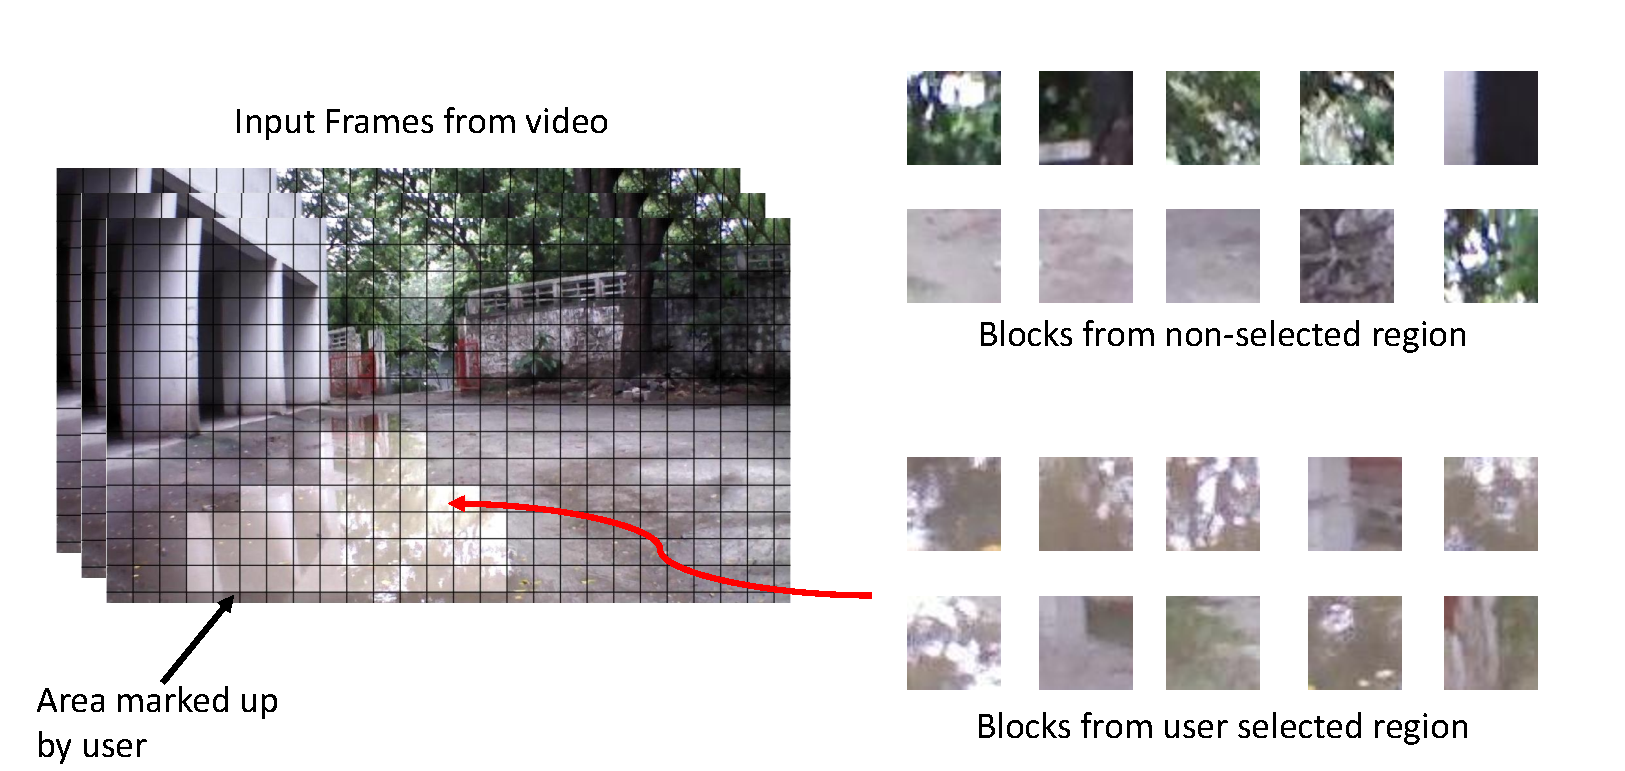
\includegraphics[width=\linewidth]{images/trainingData.pdf}
\caption{Process for creation of training data. User selects puddle area by
drawing a contour over input frame (using our tool). User can additionally
select/deselect blocks which he/she thinks are belonging to puddle/non-puddle
area. We use blocks covered by user drawn contour as `positive' training data.
While the `negative' training data is selected from blocks which are far from
the user drawn contour.}
\label{fig:training}
\end{figure}

\textbf{Failure cases of SVM :- }
The svm detector is strong at detecting regions of sky reflected off a puddle.
In the HSV color space, these regions have low saturation (S) and high
brightness (V) values, and are picked up with high reliability by the HSV
histogram feature based SVM detector. However, other reflected regions such as
trees, buildings, etc. are usually classified as non-puddle regions as these
are labeled as such in the training images.

\subsection{Optical flow based technique}
Optical flow measures apparent motion of objects in a scene caused by relative
motion between camera and object. Hence, magnitude of optical flow will be high
for near objects while objects at large distance it will be low. Figure
\ref{fig:optical_flow} shows the magitude of optical flow calculated from two images
captured from quadcopter, consisting of water puddle region. 

\begin{figure}[h!]
\centering
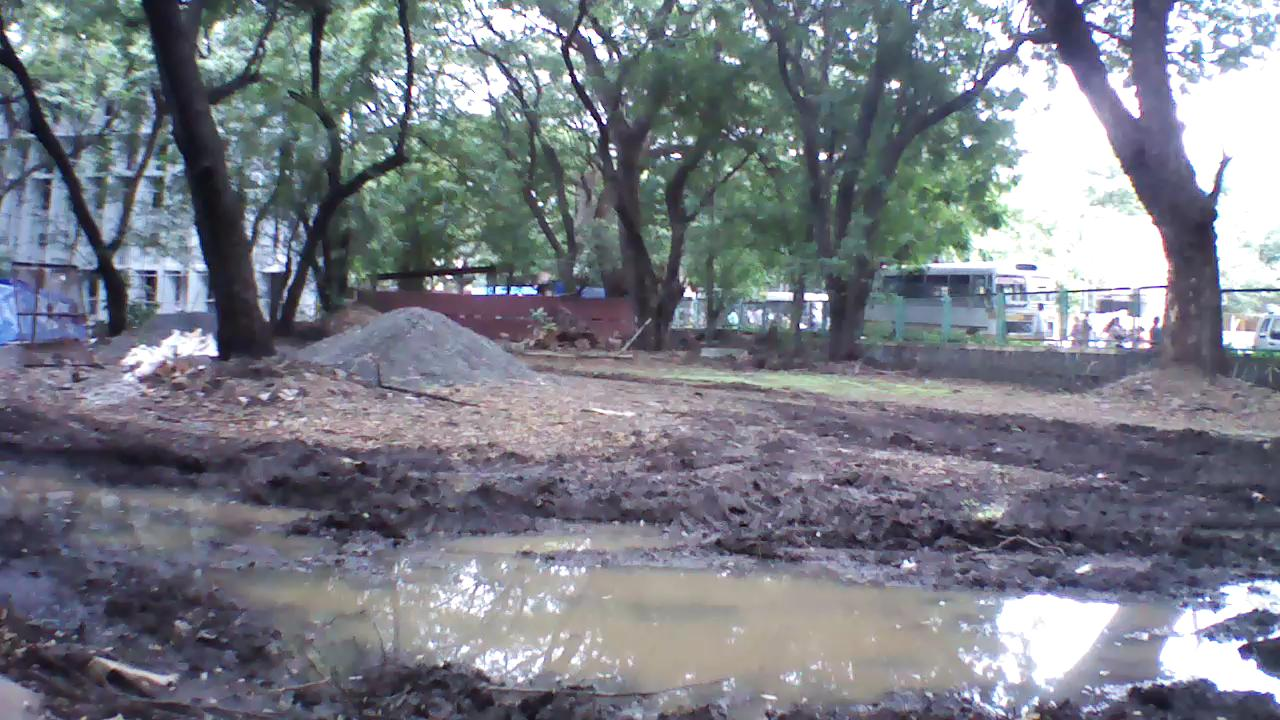
\includegraphics[width=0.3\linewidth]{images/IMG_PAIR_1_1.jpg}
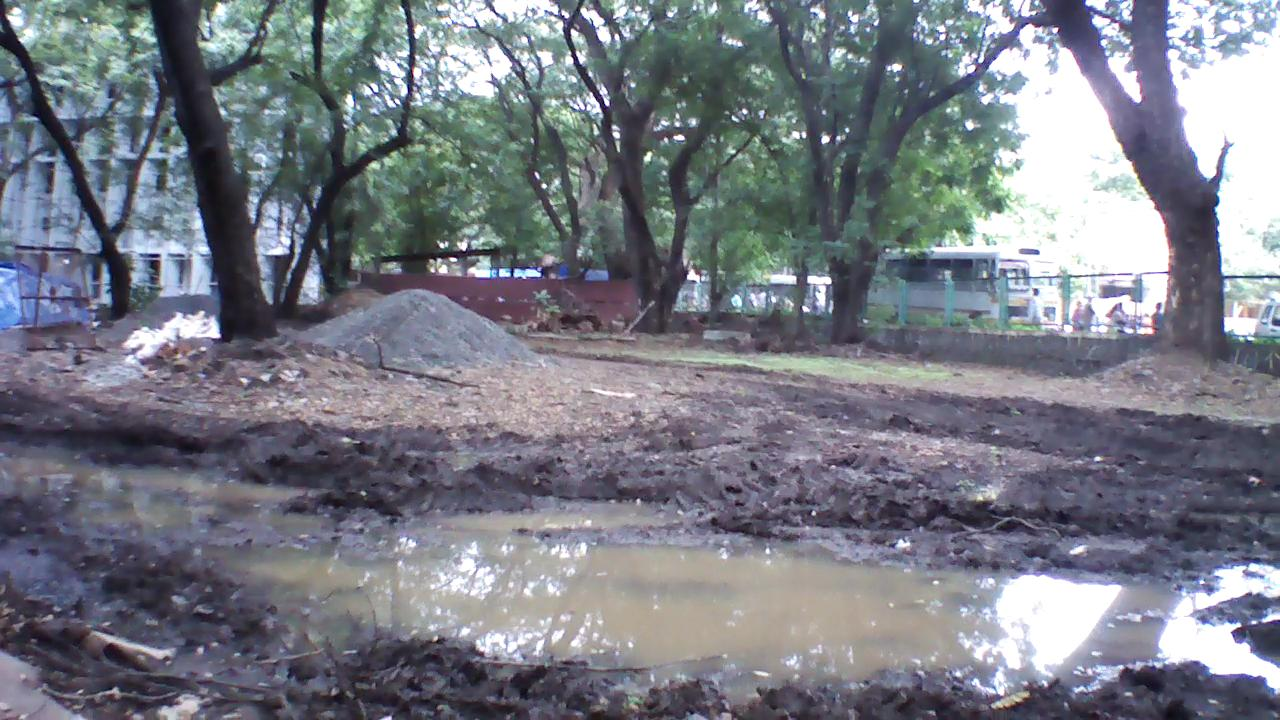
\includegraphics[width=0.3\linewidth]{images/IMG_PAIR_1_2.jpg}
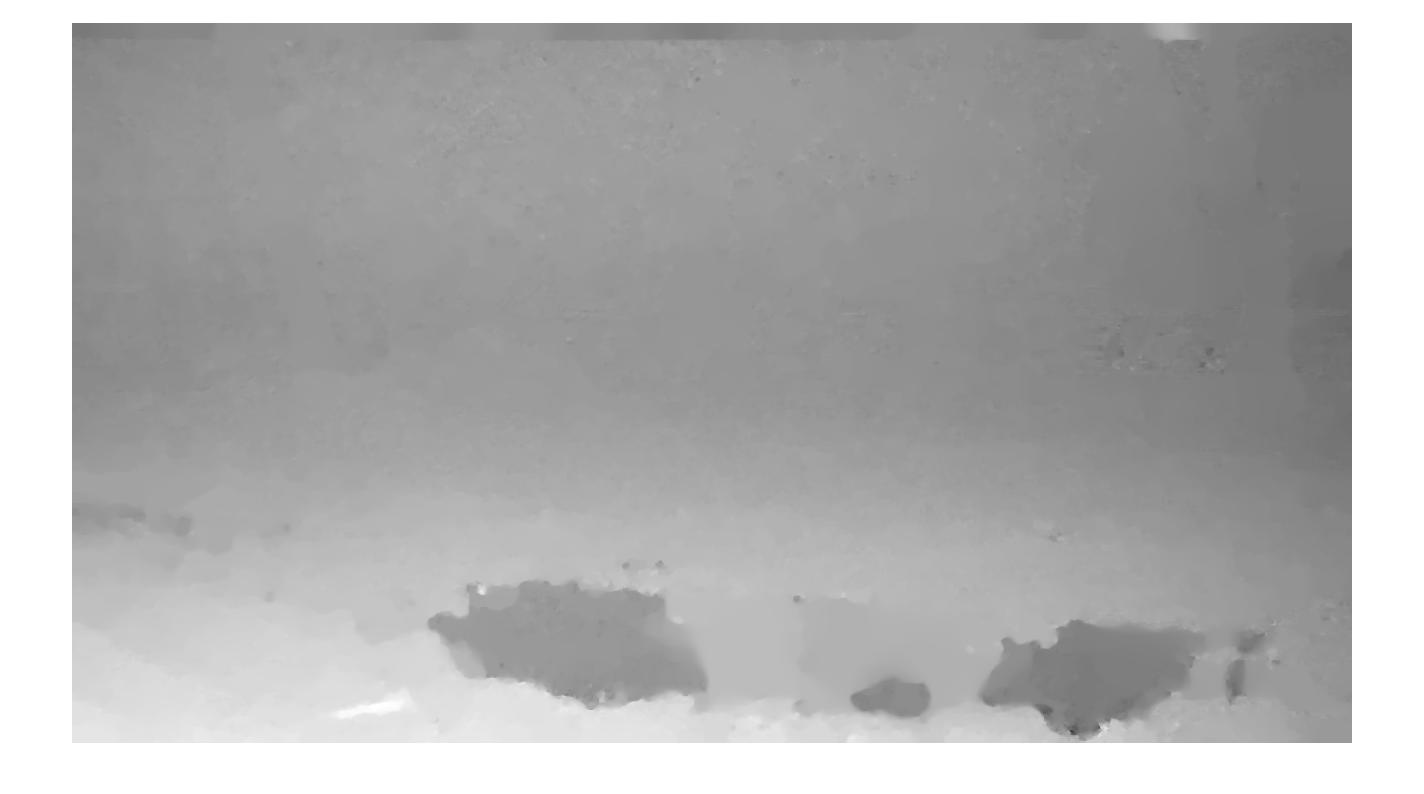
\includegraphics[width=0.3\linewidth]{images/optical_flow_magnitude.jpg}
\caption{Optical Flow. Left, middle: video frames taken from positions
which are $d$ units apart in 3D world. $ 0.01 \leq d \leq 0.1$. Right:
Magnitude of optical flow calculated from earlier images. Magnitude of optical
flow in the reflective parts of the puddle is low compared to that of its
suroundings.}
\label{fig:optical_flow}
\end{figure}

It can be seen that, the reflective part of the puddle have less optical flow
magnitude compared to its neighborhood. The reason behind this is, the reflected objects being quite far
from the actual puddle, the relative motion will be less compared to its
neighbourhood. So, we can use this property to detect water puddle regions from
the image.

We are using an algorithm  developed by Ce Liu~\cite{Liu11Thesis} which is based
on \cite{Brox04,Bruhn05} to find out optical flow. (The Matlab/C++ code for this
algorithm is given in \cite{Liu11}). \cite{Brox04} needs spatio-temporal
smoothness constraint. Temporal smoothness may be assured by taking adjacent (or
near djacent) frames from video. But, adhering to spatial smoothness constraint
is very difficult in case of UAV. 

Quadcopter provides us a way to enforce the spatial smoothness constraint on
the input images. We record Inertial Measurment Unit (IMU) data
transmitted by quadcopter, which in turn provides us the approximate position of
the quadcopter at given time. Later, we synchronize it with the video sequence
captured by quadcopter, to find out approximate position from which the given
frame is captured. Finally, we select frame pair which is nearest, among set of
temporally adjacent frames to find out the optical flow.

\textbf{Failure cases of optical flow}
Optical flow is essentially being used in a depth from parallax mode to exploit
the fact that still puddles behave like mirrors and scenery reflected by such
puddles is usually at a much greater depth than the immediate surroundings of
the puddle. Correspondingly, optical flow as a means of detecting puddles will
fail when the above assumption fails, such as when the reflected objects are
close by. Optical flow also generates false positives when the scene contains a
far off portion partially occluded by nearby objects.
 

\subsection{Combined approach}
\begin{figure}[h!]
\centering
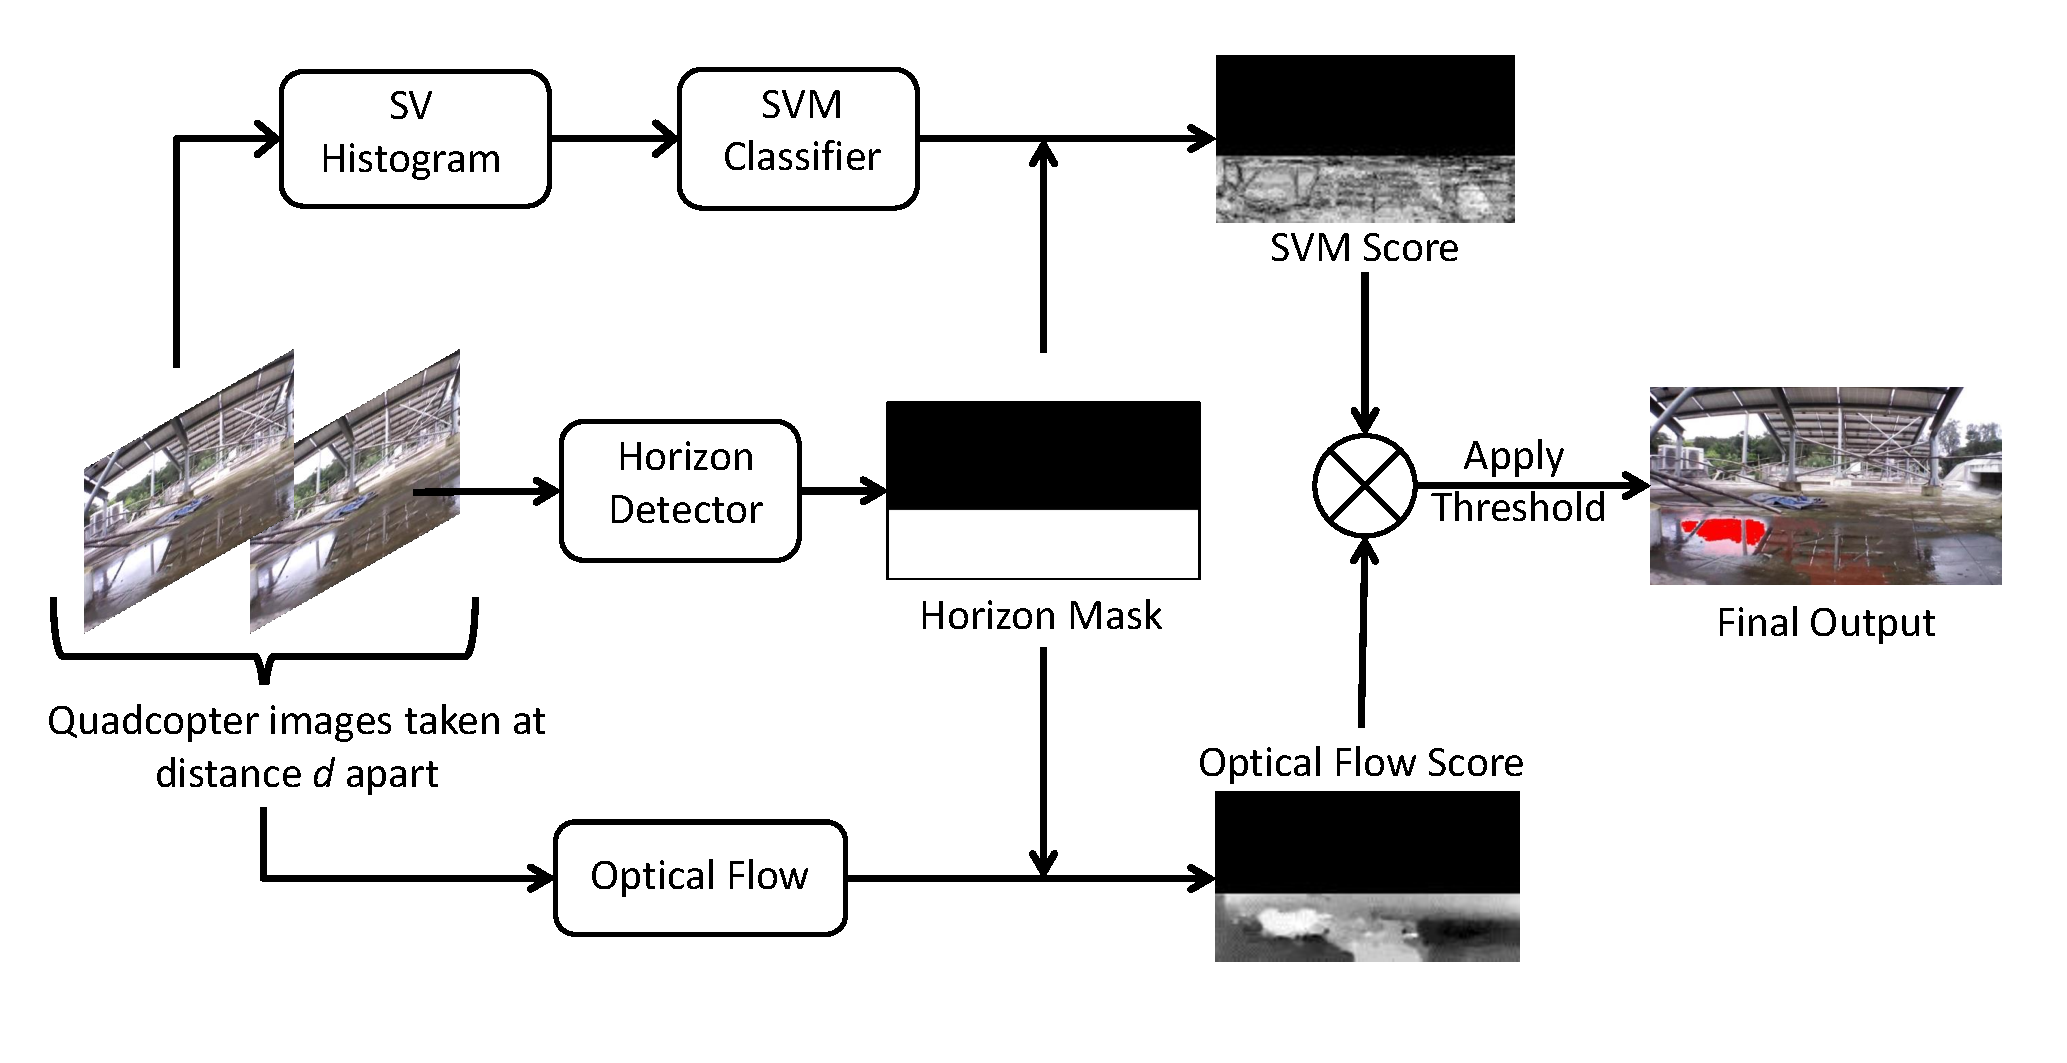
\includegraphics[width=\linewidth]{images/overall_workflow.pdf}
\caption{Overall workflow to detect stangant water.}
\label{fig:workflow}
\end{figure}

As illustrated workflow Figure \ref{fig:workflow}, intially the first image of
the input frame pair is divided into square patches. The SVM classifier is
applied to each patch and the corresponding distance from margin has been used
as a score. The given score provides a likelihood of the patch being puddle. A
grid of the scores is returned as output, which is combined with results from
optical flow stage.

\section{Experiments and Results}
\subsection{Datasets}

\subsection{Comparison with prior technique}
\subsection{Quantitative analysis}
\section{Comclusion and Future Work}

\bibliographystyle{IEEEtran}
\bibliography{egbib}
\end{document}
